\chapter{原子核的基本性质和结构}

\problem{6.1}{从 Aquila 星座方向探测到一个能量为 $10^{17}\ \mathrm{eV}$ 的宇宙线中子，试计算产生这个中子的星体离地球的最大距离。}
% layout
\answerarea

\problem{6.2}{$5\ \mathrm{MeV}$ $\alpha$ 粒子在充 $1\ \mathrm{atm}$ 空气的云室内显出 $4\ \mathrm{cm}$ 长径迹，大约要观察多少个径迹才可能有一次机会发现由于与核碰撞引起的大角弯折？}
% layout
\answerarea
\newpage

\problem{6.3}{一个 $\pi^-$ 介子最初被氘核束缚在最低的库仑轨道上，然后被氘核俘获形成一对中子，$\pi^-$ 的 $I^P=0^-$。求：
\begin{enumerate}
\item 中子对系统的总角动量和宇称；
\item 它们的轨道角动量；
\item 它们的总自旋角动量。
\end{enumerate}}
% layout
\answerarea

\newpage

\problem{6.4}{氢核自旋为 $1/2$，氘核自旋为 $1$。
\begin{enumerate}
\item 确定 H$_2$、D$_2$ 和 HD 分子的可能核自旋态；
\item 它们各自的核自旋态允许的转动态；
\item 估计 H$_2$ 分子前两个转动能级的能量差、核动能贡献的近似值、两核自旋作用及核与轨道相互作用的贡献；
\item 用（3）的结果得出 H$_2$、D$_2$ 和 HD 在温度为 $1\ \mathrm K$ 时的核自旋态分布。
\end{enumerate}}
% layout
\answerarea
\newpage

\problem{6.5}{一块石蜡样品被置于均匀磁场 $B$ 中，样品包含了许多氢原子核。
\begin{enumerate}
\item 当温度为 $T$ 时，给出处于不同磁量子数状态的质子数表达式；
\item 为观测由振动磁场产生的共振吸收，引入一个射频线圈，问它相对于稳恒磁场 $B$ 的方向应如何放置？为什么？
\item 在什么频率下可以观测到共振吸收？给出表达式。
\end{enumerate}}
% layout
\answerarea

\problem{6.6}{核磁共振计算机断层照相机（NMR--CT）是临床医学中诊断人体疾病的最新一代装置。现有一台 $400\ \mathrm{MHz}$ 的 NMR--CT。
\begin{enumerate}
\item 求所用的超导磁铁的磁感应强度；
\item 求质子能级的超精细分裂大小；
\item 要得到 $^{17}\mathrm O$ 的共振信号，频率要调到多大？（已知 $^{17}\mathrm O$ 的 $I=5/2$，$\mu=-1.89\mu_N$。）
\end{enumerate}}
% layout
\answerarea
\newpage

\problem{6.7}{\begin{enumerate}
\item 估计两个氘核聚合成 $^4\mathrm{He}$ 放出的能量及 $1\ \mathrm g$ $^2\mathrm H$ 全部聚合放出的能量。
\item 一个 $10^7\ \mathrm{kW}$ 的聚变堆每秒聚变的氘核数是多少？一年要消耗多少千克的氘？（设效率为 $100\%$。）
\end{enumerate}}
% layout
\answerarea

\problem{6.8}{计算 $^{17}\mathrm O$ 核的结合能、比结合能和最后一个中子的结合能。}
% layout
\answerarea
\newpage

\problem{6.9}{在铍核内每个核子的平均结合能为 $6.45\ \mathrm{MeV}$，氦核内为 $7.06\ \mathrm{MeV}$，要把 $^9\mathrm{Be}$ 分为两个 $\alpha$ 粒子和一个中子需消耗多少能量？}
% layout
\answerarea

\problem{6.10}{\begin{enumerate}
\item 试由原子核结合能半经验公式推出 $\beta$ 稳定线上的原子核的 $Z$ 和 $A$ 所满足的关系式。铅的 $Z=82$，求最稳定的铅的 $A$ 值。
\item 如果电耦合常数 $e^2$ 的大小为现在数值的一半，强作用不变，问 $\beta$ 稳定线怎样变化？铅的稳定质量数 $A$ 变为多少？
\end{enumerate}}
% layout
\answerarea
\newpage

\problem{6.11}{如果核力与电荷无关，np 可组成束缚态氘核，为什么不存在双中子和双质子的束缚态？}
% layout
\answerarea

\problem{6.12}{已知氘核基态角动量 $I=1$，$\mu_d=0.85744\mu_N$，$\mu_p=2.79285\mu_N$，$\mu_n=-1.91304\mu_N$。试分析氘核基态特性，为什么无 P、G 态贡献？计算纯 D 态磁矩，确定 S 态与 D 态的混合比。}
% layout
\answerarea
\newpage

\problem{6.13}{\begin{enumerate}
\item 由壳模型确定 $^{15}\mathrm O$、$^{16}\mathrm O$ 和 $^{17}\mathrm O$ 基态的 $I^P$ 值。
\item 确定 \nucl{18}{4}{F} 的 $I^P$ 值；
\item 解释偶--偶核的 $I^P$ 为什么总为 $0^+$；
\item 确定 \nucl{13}{5}{B}、\nucl{13}{6}{C} 和 \nucl{13}{7}{N} 的基态的 $I^P$；
\item 讨论这三个核的质量的相对大小，并估算 \nucl{13}{6}{C} 和 \nucl{13}{7}{N} 的质量差。
\end{enumerate}
\sourcenote{已按补充截图核对。第（2）问原图写作 $^{18}_{4}\mathrm F$，下标与元素符号不一致，这里保留原图写法，疑为原书排印错误。}}
\answerarea\newpage

\problem{6.14}{由中子单粒子壳层模型能级图，估算：
\begin{enumerate}
\item $^{207}\mathrm{Pb}$ 基态和三个最低激发态的自旋和宇称；
\item $^{209}\mathrm{Pb}$ 基态与第一激发态的自旋和宇称；
\item $^{208}\mathrm{Pb}$ 和 $^{209}\mathrm{Pb}$ 基态的磁矩；
\item $^{208}\mathrm{Pb}$ 和 $^{207}\mathrm{Pb}$ 基态的电四极矩。
\end{enumerate}
\begin{center}
\resizebox{!}{150mm}{% 根据补充的壳层模型能级图重绘。纵向位置仅作示意，不代表能量比例。
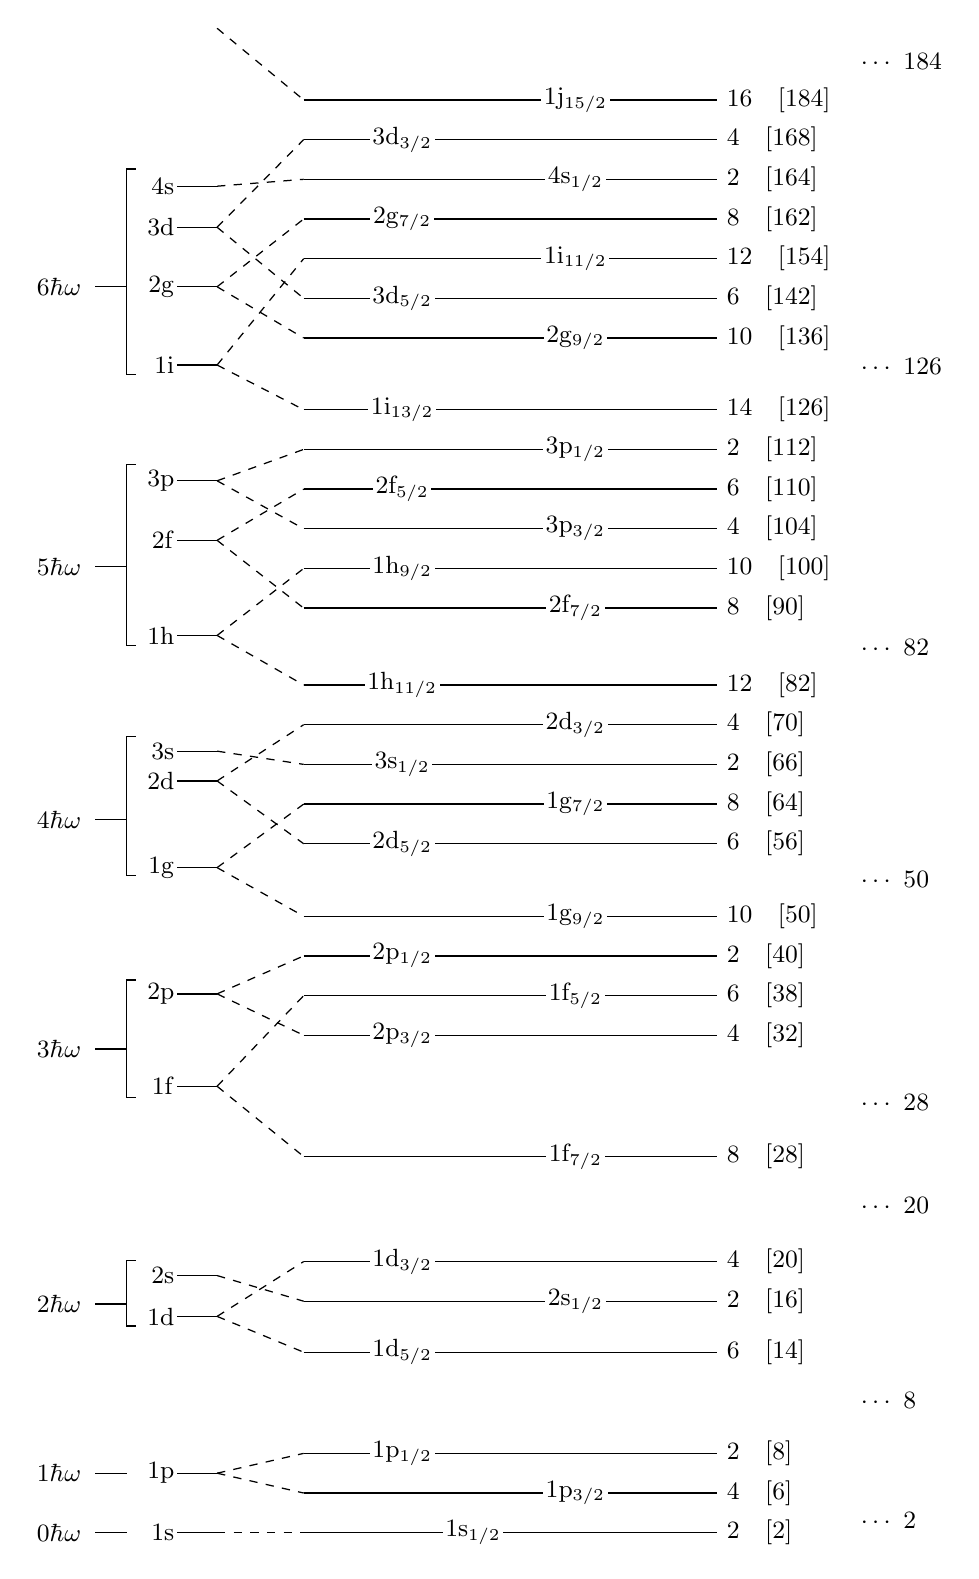
\begin{tikzpicture}[x=1cm,y=.70cm,font=\small,line width=.45pt]
\newcommand{\shelllevel}[4]{%
  \draw (3.25,#1)--(8.5,#1);
  \node[fill=white,inner sep=1pt] at (#2,#1) {$#3$};
  \node[anchor=west,fill=white,inner sep=1pt] at (8.58,#1) {$#4$};}
\newcommand{\leftlevel}[2]{\draw (1.63,#1)--(2.15,#1);\node[anchor=east,fill=white,inner sep=1pt] at (1.65,#1) {$#2$};}
\newcommand{\branch}[2]{\draw[dashed] (2.15,#1)--(3.25,#2);}
% 单粒子能级、简并度及累积核子数（由低到高）。
\shelllevel{0}{5.4}{1\mathrm s_{1/2}}{2\quad[2]}
\shelllevel{0.72}{6.7}{1\mathrm p_{3/2}}{4\quad[6]}
\shelllevel{1.44}{4.5}{1\mathrm p_{1/2}}{2\quad[8]}
\shelllevel{3.275}{4.5}{1\mathrm d_{5/2}}{6\quad[14]}
\shelllevel{4.2}{6.7}{2\mathrm s_{1/2}}{2\quad[16]}
\shelllevel{4.92}{4.5}{1\mathrm d_{3/2}}{4\quad[20]}
\shelllevel{6.825}{6.7}{1\mathrm f_{7/2}}{8\quad[28]}
\shelllevel{9.025}{4.5}{2\mathrm p_{3/2}}{4\quad[32]}
\shelllevel{9.745}{6.7}{1\mathrm f_{5/2}}{6\quad[38]}
\shelllevel{10.465}{4.5}{2\mathrm p_{1/2}}{2\quad[40]}
\shelllevel{11.185}{6.7}{1\mathrm g_{9/2}}{10\quad[50]}
\shelllevel{12.5}{4.5}{2\mathrm d_{5/2}}{6\quad[56]}
\shelllevel{13.22}{6.7}{1\mathrm g_{7/2}}{8\quad[64]}
\shelllevel{13.94}{4.5}{3\mathrm s_{1/2}}{2\quad[66]}
\shelllevel{14.66}{6.7}{2\mathrm d_{3/2}}{4\quad[70]}
\shelllevel{15.38}{4.5}{1\mathrm h_{11/2}}{12\quad[82]}
\shelllevel{16.775}{6.7}{2\mathrm f_{7/2}}{8\quad[90]}
\shelllevel{17.495}{4.5}{1\mathrm h_{9/2}}{10\quad[100]}
\shelllevel{18.215}{6.7}{3\mathrm p_{3/2}}{4\quad[104]}
\shelllevel{18.935}{4.5}{2\mathrm f_{5/2}}{6\quad[110]}
\shelllevel{19.655}{6.7}{3\mathrm p_{1/2}}{2\quad[112]}
\shelllevel{20.375}{4.5}{1\mathrm i_{13/2}}{14\quad[126]}
\shelllevel{21.675}{6.7}{2\mathrm g_{9/2}}{10\quad[136]}
\shelllevel{22.395}{4.5}{3\mathrm d_{5/2}}{6\quad[142]}
\shelllevel{23.115}{6.7}{1\mathrm i_{11/2}}{12\quad[154]}
\shelllevel{23.835}{4.5}{2\mathrm g_{7/2}}{8\quad[162]}
\shelllevel{24.555}{6.7}{4\mathrm s_{1/2}}{2\quad[164]}
\shelllevel{25.275}{4.5}{3\mathrm d_{3/2}}{4\quad[168]}
\shelllevel{25.995}{6.7}{1\mathrm j_{15/2}}{16\quad[184]}
% 未计入自旋--轨道耦合时的轨道组及其分支。
\leftlevel{0}{1\mathrm s}\branch{0}{0}
\leftlevel{1.08}{1\mathrm p}\branch{1.08}{0.72}\branch{1.08}{1.44}
\leftlevel{3.925}{1\mathrm d}\branch{3.925}{3.275}\branch{3.925}{4.92}
\leftlevel{4.6659}{2\mathrm s}\branch{4.6659}{4.2}
\leftlevel{8.1}{1\mathrm f}\branch{8.1}{6.825}\branch{8.1}{9.745}
\leftlevel{9.7763}{2\mathrm p}\branch{9.7763}{9.025}\branch{9.7763}{10.465}
\leftlevel{12.067}{1\mathrm g}\branch{12.067}{11.185}\branch{12.067}{13.22}
\leftlevel{13.64}{2\mathrm d}\branch{13.64}{12.5}\branch{13.64}{14.66}
\leftlevel{14.18}{3\mathrm s}\branch{14.18}{13.94}
\leftlevel{16.2794}{1\mathrm h}\branch{16.2794}{15.38}\branch{16.2794}{17.495}
\leftlevel{18.005}{2\mathrm f}\branch{18.005}{16.775}\branch{18.005}{18.935}
\leftlevel{19.085}{3\mathrm p}\branch{19.085}{18.215}\branch{19.085}{19.655}
\leftlevel{21.1854}{1\mathrm i}\branch{21.1854}{20.375}\branch{21.1854}{23.115}
\leftlevel{22.605}{2\mathrm g}\branch{22.605}{21.675}\branch{22.605}{23.835}
\leftlevel{23.685}{3\mathrm d}\branch{23.685}{22.395}\branch{23.685}{25.275}
\leftlevel{24.4298}{4\mathrm s}\branch{24.4298}{24.555}
\draw[dashed] (2.15,27.295)--(3.25,25.995);
% 谐振子主壳层；括号只标明归组，不表示比例。
\node[anchor=east] at (.55,0) {$0\hbar\omega$};\draw (.6,0)--(1,0);
\node[anchor=east] at (.55,1.08) {$1\hbar\omega$};\draw (.6,1.08)--(1,1.08);
\foreach \low/\high/\mid/\n in {3.75/4.9416/4.15/2,7.9/10.0267/8.775/3,11.9227/14.45/12.9383/4,16.0959/19.385/17.525/5,21.0166/24.7428/22.605/6}{
  \draw (1.12,\low)--(1,\low)--(1,\high)--(1.12,\high);
  \draw (.6,\mid)--(1,\mid);\node[anchor=east] at (.55,\mid) {$\n\hbar\omega$};}
% 壳层闭合数。
\foreach \y/\n in {0.2304/2,2.4023/8,5.9374/20,7.8/28,11.8585/50,16.0591/82,21.1516/126,26.695/184}{
  \node[anchor=west] at (10.2,\y) {$\cdots\ \n$};}
\end{tikzpicture}
}\par
\smallskip{\footnotesize 习题 6.14 图\quad 中子单粒子壳层模型能级示意图}\par
{\footnotesize 右侧分别为能级容纳数及方括号内的累积数；纵向间距不表示能量比例。}
\end{center}}
\answerarea\newpage

\problem{6.15}{\begin{enumerate}
\item 试确定 \nucl{91}{39}{Y} 核的基态和第一激发态的 $I^P$ 值；
\item 估算此原子的处于 $n=1$ 态的电子的能量；
\item 若核的第一激发能为 $555.6\ \mathrm{keV}$，它发出的 $\gamma$ 射线产生的 K 壳层光电子的动能是多少？
\item 随后发出的 K X 射线的能量是多少？
\end{enumerate}}
% layout
\answerarea
\newpage

